\documentclass[11pt]{article}
\usepackage[margin=0.85in]{geometry}
\usepackage[UTF8,fontset=fandol]{ctex}
\usepackage{amsmath,amssymb,booktabs,longtable,array,graphicx,needspace}
\usepackage[hidelinks]{hyperref}
\renewcommand{\abstractname}{Abstract}
\renewcommand{\tablename}{Table}
\renewcommand{\figurename}{Figure}
\renewcommand{\refname}{References}
\setlength{\LTpre}{6pt}
\setlength{\LTpost}{8pt}
\raggedbottom
\setlength{\parindent}{0pt}
\setlength{\parskip}{5pt}
\setlength{\emergencystretch}{2em}
\renewcommand{\arraystretch}{1.15}
\newcommand{\R}{\mathbb{R}}
\newcommand{\resultspath}{../results}
\graphicspath{{../../../figures/iteration3/}{figures/}}
\input{\resultspath/macros.tex}
\title{Finding Similar Mandarin Texts\\Using Linear Algebra\\[6pt]
\large Iteration 3: Worked Example, Implementation and Verification}
\author{James Cottrell\\DS5020 Intro Linear Algebra \& Probability}
\date{November 21, 2026}
\begin{document}
\maketitle
\begin{abstract}
This iteration implements TF-IDF, cosine similarity and SVD by power iteration
with deflation using basic NumPy operations. It verifies a four-term worked
example, preserves the Iteration 2 two-topic simulation, and compares character
and jieba word representations of the same 300 Mandarin news documents.
The 90\%-energy rule selects \CharRank{} character directions and \WordRank{}
word directions. All \VerificationCount{} recorded deterministic checks pass.
The largest singular-value difference against NumPy is \MaxSigmaError{};
the largest reduced-cosine difference against a library SVD is \MaxCosineError.
Topic separation increases after reduction, but nearest-topic accuracy and
individual query rankings do not consistently improve. Numerical correctness
and semantic usefulness therefore require separate evaluation.
\end{abstract}

\section{Scope, continuity and ownership}
The question is how truncated SVD changes topical similarity between Mandarin
texts. This connects the project to my computer science and linguistics background.
The Iteration 2 dataset, document IDs, TF-IDF formula and seed-0 simulation are
preserved. Its Jacobi eigensolver is retained as prior work; this iteration uses
the newly required power-iteration/deflation method. Word segmentation, three
simulation sizes and an overlap stress test are additions required by the new
handout. They are identified explicitly below.

Student owner and solo project lead: James Cottrell. Preparation of code,
experiments and exposition used AI assistance. Student review and the ability
to explain the work remain James's responsibility. The handout's rotating-leader
and second-person-checker wording has no clarified solo convention. No second
student, checker signature or instructor approval is claimed. Computational
verification is documented independently of that unresolved human convention.

\section{Notation and conventions}
\begin{center}\small
\begin{tabular}{p{.22\textwidth}p{.47\textwidth}p{.22\textwidth}}
\toprule Symbol & Meaning & Size/domain\\\midrule
$m,n,k$ & Terms, documents, retained rank & Positive integers\\
$C,A$ & Count and TF-IDF matrices; terms in rows & $m\times n$\\
$df_t,w_t,q$ & Document frequency, fitted IDF, query & Scalars; $q\in\R^m$\\
$G,p$ & Smaller Gram matrix and its dimension & $p\times p$, $p=\min(m,n)$\\
$U_k,\Sigma_k,V_k$ & Retained SVD factors, $\Sigma_k=\mathrm{diag}(\sigma_i)$ & $m\times k,\ k\times k,\ n\times k$\\
$D,z,\widehat q$ & Document rows, projected query, folded query & $n\times k,\ k,\ k$\\
$Q,P,G_i$ & Found Gram directions, complementary projector, deflated Gram & $p\times i,\ p\times p,\ p\times p$\\
$h,\theta_h,L$ & Simulated topic, term distribution, document length & $h\in\{0,1\}$, $\theta_h\in[0,1]^{50}$, $L=60$\\
$p_h,N_h,\widehat p_h$ & First-half token probability, token count, estimate & Scalars\\
\bottomrule
\end{tabular}\end{center}
For vectors, $\|x\|_2=\sqrt{\sum_i x_i^2}$; for matrices,
$\|A\|_F^2=\sum_{t,j}A_{tj}^2$. No centering, smoothing, stopword list or
document-length normalization is applied before SVD. Cosines normalize
individual vectors at comparison time. This is an uncentered text
representation, not centered PCA.

\section{Iteration 3 -- Math Questions}
\subsection{Q1: Four terms, three documents and a complete SVD}
Use terms $(\text{天},\text{气},\text{足},\text{球})$ and documents
$\text{天气}$, $\text{天气足球}$, $\text{足球}$ in that order.
These are designed toy strings, not news observations.
Counting each term gives
\[
C=\begin{bmatrix}1&1&0\\1&1&0\\0&1&1\\0&1&1\end{bmatrix},
\quad df=(2,2,2,2)^\top,\quad
\alpha=\log(3/2),\quad A=\alpha C\in\R^{4\times3}.
\]
Each row occurs in two of three documents, so the common IDF is $\alpha$ by
the definition of IDF. Matrix multiplication gives
\[
G=A^\top A=\alpha^2 B,\qquad
B=\begin{bmatrix}2&2&0\\2&4&2\\0&2&2\end{bmatrix}.
\]
Expanding the determinant along the first row,
\[
\det(xI-B)=(x-2)\big((x-4)(x-2)-4\big)-4(x-2)
=x(x-2)(x-6).
\]
Thus the eigenvalues of $G$ are $6\alpha^2,2\alpha^2,0$ by scalar
multiplication of eigenvalues. Solving each homogeneous system and
normalizing by the Euclidean norm gives
\[
v_1=\frac{(1,2,1)^\top}{\sqrt6},\quad
v_2=\frac{(1,0,-1)^\top}{\sqrt2},\quad
v_0=\frac{(1,-1,1)^\top}{\sqrt3}.
\]
Their pairwise dot products vanish. The positive singular values are
$\sigma_1=\sqrt6\,\alpha$ and $\sigma_2=\sqrt2\,\alpha$ by taking positive
square roots. Using the Iteration 2 construction $u_i=Av_i/\sigma_i$ gives
\[
u_1=\tfrac12(1,1,1,1)^\top,\qquad
u_2=\tfrac12(1,1,-1,-1)^\top.
\]
These are unit and orthogonal. With $U=[u_1,u_2]$, $V=[v_1,v_2]$,
$\Sigma=\mathrm{diag}(\sigma_1,\sigma_2)$, substitution gives
$U\Sigma V^\top=A$. This is the compact rank-2 SVD; the null vector
does not supply a positive singular direction.

Rank one gives
\[
A_1=u_1\sigma_1v_1^\top
=\frac{\alpha}{2}\begin{bmatrix}1&2&1\\1&2&1\\1&2&1\\1&2&1\end{bmatrix},
\qquad D_1=\alpha(1,2,1)^\top.
\]
Every reduced document is a positive scalar in $\R^1$, so every defined
cosine is one. Originally, the first and third documents are orthogonal;
the other two distinct-document cosines are $1/\sqrt2$, by the dot-product
formula. Rank one retains $6/(6+2)=3/4$ of the energy and has squared
Frobenius error $2\alpha^2$ by the discarded-energy identity.
\input{\resultspath/tiny_cosines.tex}
This example exposes loss of distinction, even though the approximation is
optimal for its rank in Frobenius norm.

\textbf{Independent check.} \path{small_example.py} computes $C^\top C$
with \texttt{Fraction}, evaluates $Gv_i-\sigma_i^2v_i$ and $Gv_0$,
checks $U^\top U=V^\top V=I$, substitutes the factors back into $A$,
and compares the error with $2\alpha^2$. It also runs the shared power
solver and the library checks. Counts and rational products are exact;
logarithms and square roots are stated symbolically and evaluated in
floating point. Appendix A prints the numerical matrices; Appendix B
lists every power iterate. The script prints all stages, including
the starting vectors and convergence diagnostics.

\subsection{Q2: From-scratch functions and their equations}
The shared numerical core is \texttt{src/methods.py}. Every function below
has an equation comment, and the same functions run the tiny example,
the simulation and the real corpus. NumPy's decomposition solvers and
scikit-learn are used only in verification helpers.

\textbf{Steps 1--2: counts and weighting.}
\begin{align}
C_{tj}&=\sum_{x\text{ in document }j}\mathbf1\{x=t\},
&& C\in\R^{m\times n}. \tag{E1}\\
df_t&=\sum_j\mathbf1\{C_{tj}>0\},\quad
w_t=\log(n/df_t),\quad A_{tj}=C_{tj}w_t. \tag{E2}\\
q_t&=C^{\mathrm{query}}_t w_t,
&&q\in\R^m. \tag{E3}
\end{align}
These are \path{my_count_matrix}, \path{my_tfidf} and
\path{my_query_vector}. An unobserved fixed-vocabulary row gets weight
zero without evaluating $\log0$. Queries reuse the fitted vocabulary/IDF.

\textbf{Steps 3--5: Gram matrix, power iteration and deflation.}
\begin{align}
G&=\begin{cases}A^\top A&n\le m\\AA^\top&m<n,\end{cases}
&&G\in\R^{p\times p}. \tag{E4}\\
P_i x&=(I-Q_iQ_i^\top)x,
&&Q_i\in\R^{p\times i}. \tag{E5}\\
x_{\ell+1}&=\frac{P_iG_i x_\ell}{\|P_iG_i x_\ell\|_2},\quad
\lambda=x_{\ell+1}^\top Gx_{\ell+1}. \tag{E6}\\
G_{i+1}&=G_i-\lambda vv^\top,\quad G_0=G. \tag{E7}\\
\sigma_i&=\sqrt{\lambda_i},\qquad
u_i=Av_i/\sigma_i\ \text{(right Gram)},\quad
v_i=A^\top u_i/\sigma_i\ \text{(left Gram)}. \tag{E8}
\end{align}
These correspond to \path{my_gram}, \path{my_reorthogonalize},
\path{my_power_iteration}, \path{my_deflate} and
\path{my_svd_power}. Two passes of (E5) reduce loss of orthogonality.
The smaller left Gram is used for the 50-term simulations when $n>50$;
the right Gram is used for the toy and real matrices.
Both routes are justified by the Iteration 2 SVD-construction proof.

To see why power iteration finds a leading direction, expand
$x_0=\sum_j c_jv_j$ in an orthonormal eigenbasis. Then
$G^\ell x_0=\lambda_1^\ell(c_1v_1+
\sum_{j>1}c_j(\lambda_j/\lambda_1)^\ell v_j)$ by the eigenvector equation.
If $c_1\ne0$ and $\lambda_1>\lambda_2$, normalization suppresses the
other components at a rate controlled by $\lambda_2/\lambda_1$.
For $A^\top A$ this is $(\sigma_2/\sigma_1)^2$.
Deflation works because
$(G-\lambda_1v_1v_1^\top)v_1=0$ and, for $j>1$,
$(G-\lambda_1v_1v_1^\top)v_j=\lambda_jv_j$ by orthogonality.
Repeated values identify a subspace rather than a unique vector.

The fixed starting RNG has seed 0. The stopping test is a projected
deflated-Gram eigen-residual at most $10^{-14}\|G\|_F$, with a maximum
of 200,000 iterations per direction. The original-Gram residual is
also recorded. Eigenvalues at or below $10^{-12}$ of the leading
value are rejected as unresolved, consistent with the earlier cutoff.
Failure to converge or to resolve a positive value raises an error.
Gram construction squares the nonzero condition number and therefore
requires this numerical caution.

\textbf{Steps 6--8: coordinates, similarities, energy and ordering.}
\begin{align}
D&=V_k\Sigma_k\in\R^{n\times k}. \tag{E9}\\
z&=U_k^\top q,\qquad \widehat q=\Sigma_k^{-1}z\in\R^k. \tag{E10}\\
N_i&=X_i/\|X_i\|_2,\qquad S=NN^\top. \tag{E11}\\
s_j&=\frac{D_j^\top z}{\|D_j\|_2\|z\|_2}. \tag{E12}\\
E_k&=\frac{\sum_{i=1}^k\sigma_i^2}{\|A\|_F^2},\qquad
k_*=\min\{k:E_k\ge0.90\}. \tag{E13}\\
\mathrm{matches}&=\text{five largest }s_j\text{ after self-ID exclusion}. \tag{E14}
\end{align}
Ascending ID breaks score ties. These map to
\path{my_document_coordinates}, \path{my_project_query},
\path{my_normalize_rows}, \path{my_cosine_matrix},
\path{my_query_cosines}, \path{my_energy_rank} and
\path{my_top_matches}.

For a document $q=Ae_j$, $U_k^\top q=\Sigma_kV_k^\top e_j$
by orthonormality. Thus the projected query matches row $j$ of $D$,
and the folded query matches row $j$ of $V_k$.
Retrieval compares $z$ with $D$; the fold-in identity compares
$\widehat q$ with $V_k$. Unequal diagonal scaling changes angles.

Counts cost $O(T+mn)$ for $T$ tokens and a dense matrix; TF-IDF costs
$O(mn)$. The smaller Gram costs $O(mnp)$. Direction $i$ costs
$O(t_i(p^2+pi))$ for $t_i$ power steps and reorthogonalization.
Deriving opposite-side factors costs $O(mnk)$. All-pairs cosine costs
$O(n^2k)$ after reduction, compared with $O(n^2m)$ before it.
Working storage is $O(mn+p^2+(m+n)k)$, plus any cosine matrix.

\subsection{Q3: Rank from real-data energy}
The predeclared choice is the smallest rank retaining 90\% of squared
singular-value energy, independently for each tokenization.
This percentage is an analysis choice; the Mandarin handout does not
prescribe one. The identity $\|A\|_F^2=\sum_i\sigma_i^2$
(from orthogonal invariance of the Frobenius norm) supplies the denominator.
The custom solver extracts successive directions until the target is met;
a full NumPy spectrum verifies the result afterward.
\input{\resultspath/real_shapes.tex}
For characters, $E_{\CharRank}=\CharEnergy$ and the previous energy is
\CharPreviousEnergy. For words, $E_{\WordRank}=\WordEnergy$ and the
previous energy is \WordPreviousEnergy. Hence the reported ranks are
minimal for this threshold. The Frobenius tail identity gives
$\|A-A_k\|_F^2/\|A\|_F^2=1-E_k$.
Retaining energy controls squared reconstruction loss, not relevance.
The fairly high ranks reflect lexical variation beyond the few topic labels.
The next/last-retained singular-value ratios are \CharBoundaryRatio{}
and \WordBoundaryRatio{}, so convergence near the cutoff is slower than
for a widely separated leading direction.
\begin{figure}[htbp]\centering
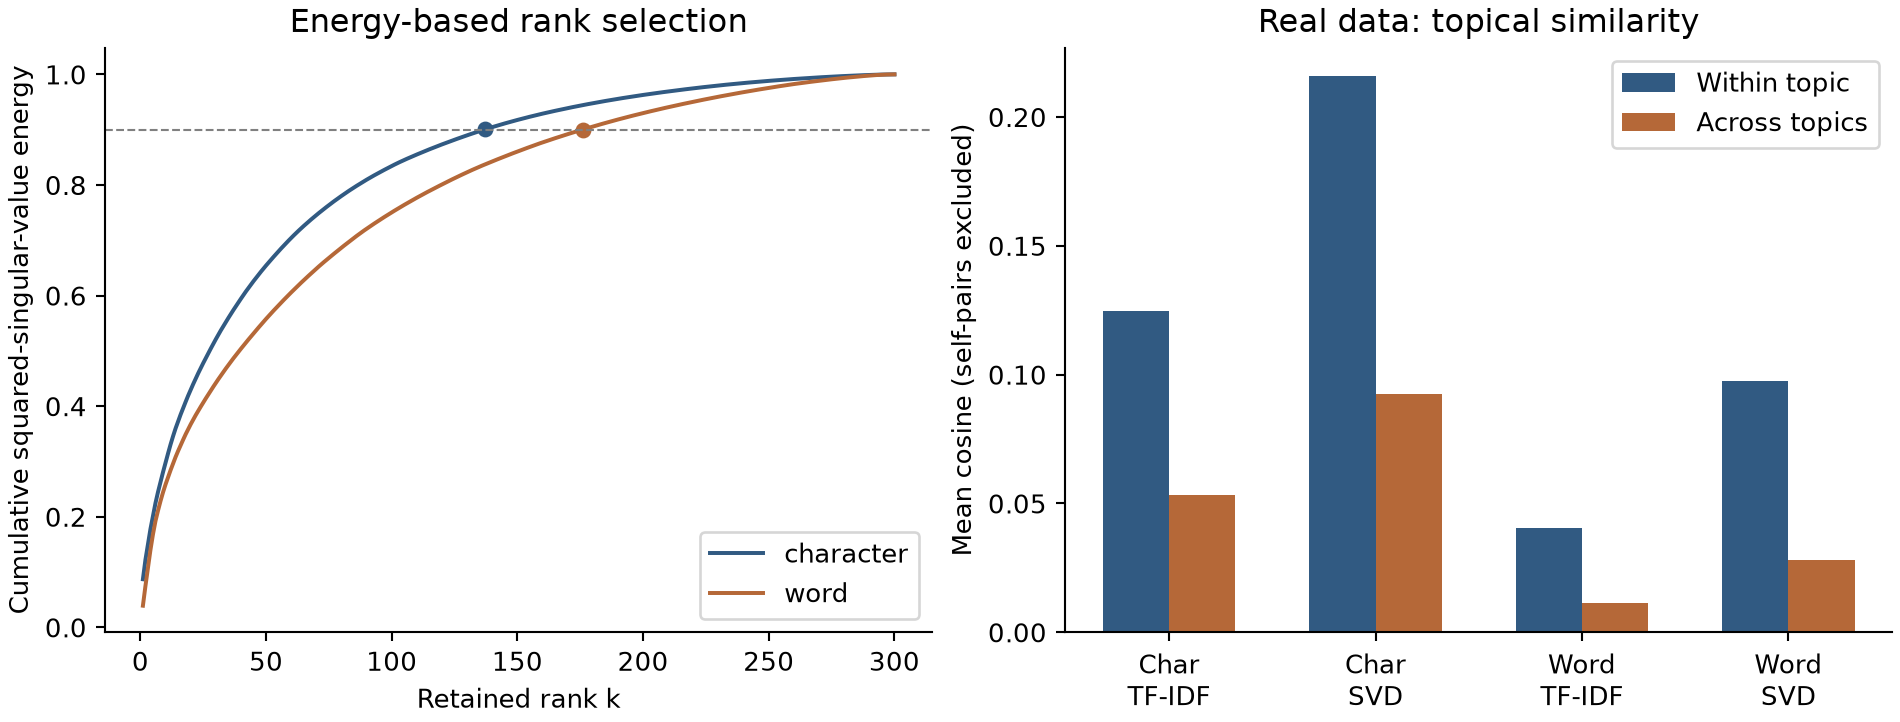
\includegraphics[width=\textwidth]{real_comparison.png}
\caption{Left: full reference energy curves, with custom-selected ranks marked.
Right: measured topic means from the custom representations.}\end{figure}

\subsection{Q4: Characters versus jieba words}
Both representations use exactly the same 300 document IDs and the same
raw-TF/unsmoothed-IDF rule. Character filtering keeps U+4E00--U+9FFF,
as in Iteration 2. Word preprocessing replaces discarded runs by spaces
to preserve boundaries, then uses jieba 0.42.1 precise mode,
\path{cut_all=False}, \texttt{HMM=True}, and its default dictionary.
Only fully Chinese tokens are retained. No stopword list or minimum
frequency is added. The word vocabulary is larger and its matrix is sparser.
\input{\resultspath/real_similarity.tex}
Within/across topic means both rise after SVD, while their difference
also rises. Character nearest-topic agreement is unchanged; word
nearest-topic agreement falls after reduction.
The original word representation has the strongest nearest-topic
agreement among these four settings, despite smaller raw cosines.
Absolute cosines are not directly comparable across different feature
spaces. Each representation has its own energy-selected rank, so the
comparison combines tokenization with the rank implied by the common rule.
Topic labels are a useful proxy, not a judgment of semantic equivalence.

\subsection{Q5: One fixed query and its top five matches}
The query is the full title/body of the first document in the unchanged
sample manifest, \texttt{sports:2}, titled
“冠军球队迎新欢乐派对 黄旭获大奖张军赢下PK赛”.
It describes a golf-party event involving champion athletes.
The choice was fixed before inspecting rankings. Its own ID is excluded.
This is descriptive in-corpus retrieval, with no held-out evaluation.
\input{\resultspath/query_character_original.tex}
\input{\resultspath/query_character_reduced.tex}
The original character ranking puts an education interview first.
The largest positive dot-product terms include individual name characters
such as 煊, 张 and 伟 (recorded in \path{query_term_contributions.csv}).
Such overlaps can connect unrelated names and contexts.
After reduction, \texttt{sports:374} moves from fourth to first, but it
is a basketball report rather than the same golf event.
Some education results remain. The change in angles is real;
the ranking does not establish improved semantic relevance.
\input{\resultspath/query_word_original.tex}
\input{\resultspath/query_word_reduced.tex}
Original word matches include sports reports sharing terms such as
冠军 and 球队. The reduced word ranking contains no sports-labeled
document in its top five. Its first result concerns an event for returning
overseas scholars. Shared broad event language can coexist with a wrong
topic, and projection spreads term weights through the retained subspace.
Terms highlighted from a reconstructed vector need not occur literally
in that article. These results illustrate why energy preservation and
numerical correctness do not guarantee a useful query ranking.
No query or rank was changed to hide this failure case.

\clearpage
\section{Simulation: truth, numerical agreement and stress}
\subsection{Preserved model and sample-size experiment}
The original generator uses \path{default_rng(0)}. First it draws
$\theta_0\sim\mathrm{Dirichlet}(2,\ldots,2,0.1,\ldots,0.1)$ with
25 entries in each group, then $\theta_1$ with the two groups reversed.
For each topic $h$, documents are independent
$\mathrm{Multinomial}(60,\theta_h)$ count columns, conditional on
the drawn probabilities. Topic-0 documents are generated first.
At $n=40$, there are 20 documents per topic.
The new \path{simulate_two_topics} function returns counts, labels,
probabilities and settings, and reproduces the saved Iteration 2
counts, labels and probabilities exactly.

Additional balanced sizes are $n=200$ and $1000$, with the same seed,
realized probabilities and document length. These extensions satisfy
the new requirement for at least three sizes. They are not nested for
topic 1 because the number of earlier topic-0 draws changes.
The observed noisy TF-IDF matrix is not asserted to have rank two.
All sizes use the shared custom method at $k=2$.
\input{\resultspath/simulation_similarity.tex}
The handout's baseline test includes self-pairs in its within-topic mean.
That statistic also passes $>0.9$, with across-topic mean $<0.2$.
The table uses the stricter off-diagonal within-topic mean for interpretation.
Both representations already attain perfect nearest-topic agreement
in this separated baseline, so no accuracy gain is claimed.

\subsection{Known-probability sampling error}
The Mandarin box uses topic labels as truth. In addition to label
recovery, the general error-versus-$n$ requirement is addressed using
the probability statistic derived in Iteration 2. It is not an error
curve for singular vectors, whose signs and bases may differ.
Let $X_\ell$ indicate that token $\ell$ falls in the first 25 terms.
For topic $h$,
\[
p_h=\sum_{t=1}^{25}\theta_{ht},\quad
\widehat p_h=\frac{1}{N_h}\sum_{\ell=1}^{N_h}X_\ell,\quad
N_h=60(n/2).
\]
Since $X_\ell$ are independent Bernoulli variables conditional on
$\theta_h$, linearity of expectation gives
$\mathbb E[\widehat p_h\mid\theta_h]=p_h$.
Variance additivity under independence gives
\[
\mathrm{Var}(\widehat p_h\mid\theta_h)
=\frac{p_h(1-p_h)}{N_h},\qquad
SE_h=\sqrt{\frac{p_h(1-p_h)}{N_h}}.
\]
Thus the theoretical standard error decreases as $n^{-1/2}$.
\input{\resultspath/simulation_probability.tex}
All six estimates are within 3SE. A single seeded absolute error need
not decrease monotonically, and the observed curve does fluctuate.
The SE line supplies the scaling reference. No seeds were selected
to force an apparent trend. A 3SE comparison is a sampling diagnostic,
not a deterministic accuracy guarantee or a claim about real-language
token independence.
\begin{figure}[htbp]\centering
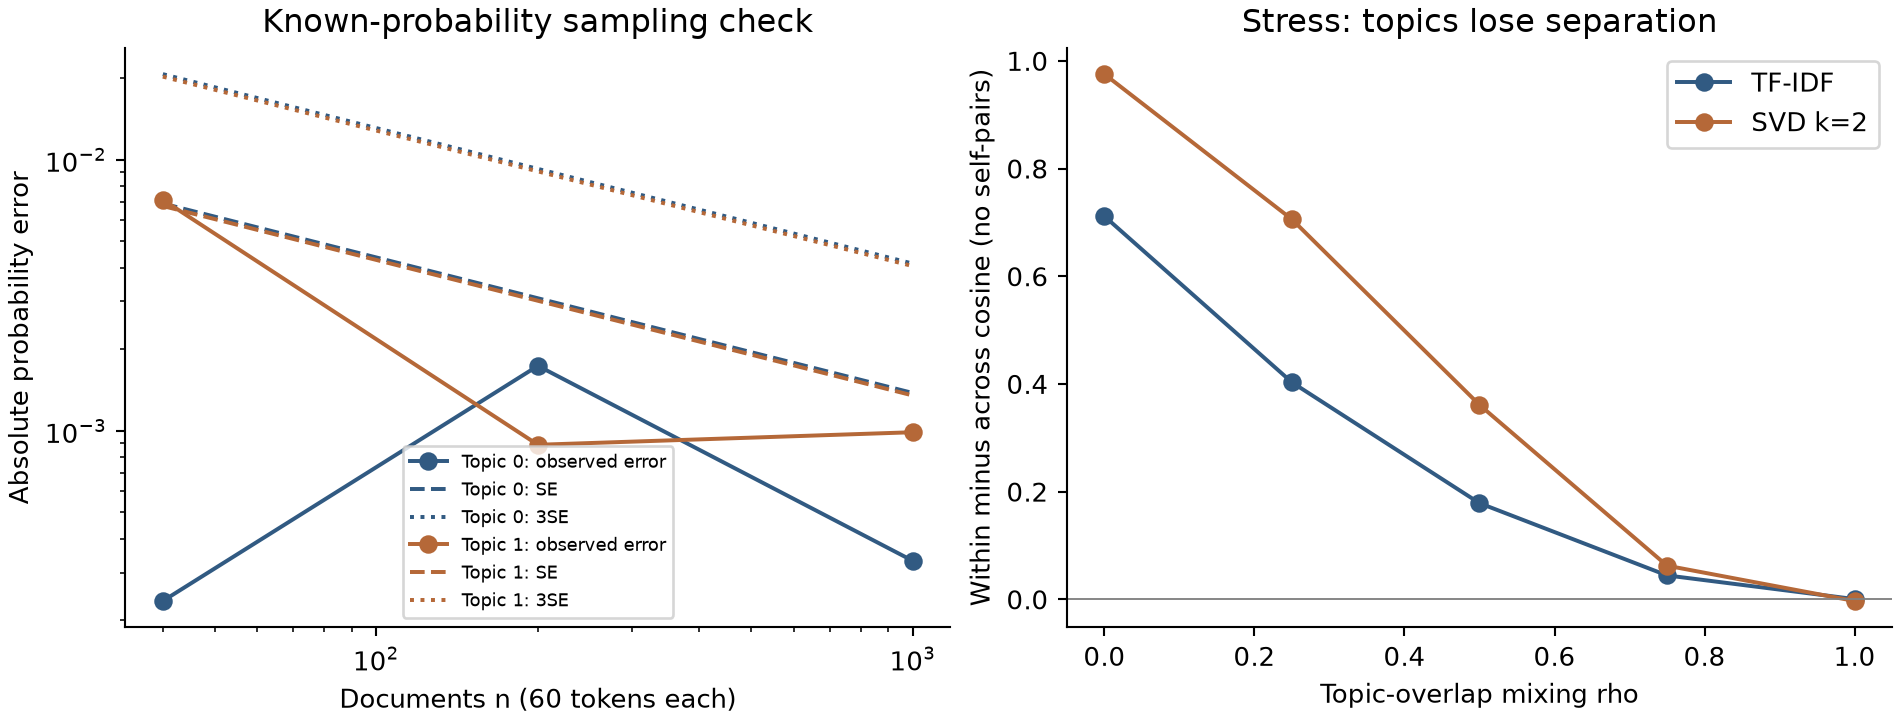
\includegraphics[width=\textwidth]{simulation_checks.png}
\caption{Known-probability error on log-log axes and the topic-overlap stress test.
SE curves are conditional on the fixed drawn topic probabilities.}\end{figure}

\subsection{Stress test: remove topic separation}
The intentional model change is
\[
\theta_h(\rho)=(1-\rho)\theta_h+
\rho(\theta_0+\theta_1)/2,\qquad
\rho\in\{0,0.25,0.5,0.75,1\}.
\]
Seed 0, $n=40$ and 60 tokens per document are retained.
At $\rho=1$, the two distributions coincide and the labels no longer
encode a distributional difference. This breaks the useful-separation
condition, not the algebraic SVD identities.
\input{\resultspath/stress.tex}
The cosine gap closes and the reduced nearest-topic rate falls.
The slightly negative final reduced gap is a finite-sample outcome.
Across-topic similarity can become large even though the numerical
library checks still pass. This is the expected limitation of the
method when topics no longer have distinguishable term distributions.

\section{Real data, cleaning and reproducibility}
The data are the same THUCNews title/body documents from the pinned
Tongjilibo mirror revision
\texttt{ae77e363396e90b54cdaa9eafdbc5e102a3d4019}.
The source prefixes each contain 1,000 records from sports, education
and technology. The original procedure retains at least 30 Chinese
characters, removes exact duplicates within each category, and samples
100 eligible documents per category with seed 0.
The new code uses the recorded IDs rather than selecting a new sample.
\input{\resultspath/cleaning.tex}
The selected title/body strings agree exactly with the local Iteration 2
document table; the character TF-IDF matrix also agrees entry for entry.
No selected document is removed in Iteration 3.
Per-document counts of discarded characters, punctuation and digits
are saved in \path{real_cleaning.csv}. Ordered character and word
token sequences are saved locally as JSONL, with dictionary/settings
and SHA-256 hashes in \texttt{tokenization.json}.
No raw corpus or full processed text is added to Git.

There is no train/test split: this experiment describes similarities
within the fixed collection and uses one of those documents as a
query. Topic labels do not enter counts, IDF or SVD. A future held-out
study would fit vocabulary/IDF using training documents only.
The finite-prefix candidate pool limits representativeness, so these
results do not establish performance on the complete THUCNews corpus.

For TF-IDF verification, scikit-learn's unsmoothed IDF still adds one.
The comparison subtracts that one before applying raw counts and
disables normalization. Comparing against default library TF-IDF
would test a different formula. SVD signs are canonicalized for
readability; reconstruction and cosine comparisons avoid sign ambiguity.
Repeated singular values require subspace comparisons rather than
entrywise equality of arbitrary eigenvectors.

\section{Assumption checks and limitations}
The numerical and frozen-vocabulary checks run on simulation first,
then real data. All recorded known queries match their fitted document
column; adding an OOV token changes no supported coordinate; a fully
unsupported query is rejected. Zero-vector cosine is never assigned
an artificial value.
\input{\resultspath/numerical_assumptions.tex}

\begin{longtable}{p{.25\textwidth}p{.65\textwidth}}
\toprule Assumption / choice & Check and interpretation\\\midrule\endhead
One vocabulary and IDF & Known/mixed-OOV/unsupported query checks pass on all
three simulated sizes and both real representations. Each tokenizer has its
own fixed feature space.\\
Nonzero original and projected vectors & Counts are recorded for both spaces.
No zero real vectors occur. Unsupported queries and explicit zero-vector
test cases raise errors.\\
Positive resolved singular values & Retained values are positive, the energy
rank agrees with a full library spectrum, and boundary ratios are reported.
A looser tolerance $10^{-13}$ changes real cosine matrices by less than
$10^{-8}$. The cutoff is a numerical policy, not proof that excluded
directions have no information.\\
Approximately orthonormal factors & U/V orthogonality, original-Gram residuals,
projection identities and reconstructed-vector cosines are measured.
The normalized Frobenius tail-identity errors pass the stated tolerance.\\
Labels as an imperfect similarity proxy & Known simulation topics give a
controlled reference. Real category means and query inspection disagree
with an unconditional improvement claim. Topic agreement is not semantic
equivalence.\\
No selected exact duplicates & Both representations have zero exact duplicates.
The highest original-cosine pairs are saved for inspection. The leading
character pair, \texttt{technology:685/686}, concerns two reports of a
failed satellite launch; related reporting can inflate neighbor scores
without being exact duplicate text. No such document is silently dropped.\\
Finite-prefix representativeness & The source manifest and original selection
procedure are preserved. No numerical test can make a prefix sample
representative of the whole corpus. The conclusion is restricted to this
fixed collection.\\
Conditional simulated-token independence & Frequencies fall within the displayed
3SE diagnostic. Independence follows from the generator, and cannot be
proved from a finite frequency check. Real text is not assumed to consist
of independent tokens.\\
\bottomrule
\end{longtable}
Bag representations discard order, syntax and compositional meaning.
Simplified/traditional variants are not merged.
Raw counts let longer documents and repeated names influence the SVD.
No stopword filtering was introduced for this comparison.
The larger word vocabulary also contains rare segmentation/name tokens.
These are substantive representation limitations even when every
numerical check passes.

\section{Unified numerical verification}
\path{verification_helpers.py} prints one consistent format and saves
max absolute differences, Frobenius relative differences, tolerance and
pass status. If a reference norm is zero, a nonzero relative difference
is left undefined rather than divided by zero.
Singular-value and cosine comparisons use an absolute $10^{-8}$ limit.
Rank-$k$ reconstruction and the tail identity are compared using
explicitly normalized errors with a $10^{-10}$ limit, avoiding a
scale-dependent test on large squared energies. No raw singular-vector
comparison assumes identical signs.

All \VerificationCount{} deterministic comparison records pass.
Additional tall, wide, rank-deficient, repeated-value, zero-input,
invalid-rank and nonconvergence cases are checked in
\path{verify_iteration3.py}. The following table includes key checks
and the separate sampling comparisons; the full records are in
\path{docs/iteration3/results/verification_all.csv}.
Every displayed difference is generated by a script.
\input{\resultspath/verification.tex}


\section{Reproduction and progress}
Run from the repository root with the pinned Python environment:
\begin{verbatim}
python src/download_data.py     # only if raw prefixes are absent
python src/small_example.py
python src/verify_iteration3.py
python src/check_simulation.py
python src/run_real.py
python src/build_iteration3_report.py
\end{verbatim}
The final build needs XeLaTeX, including \texttt{ctex}/Fandol for Chinese.
The Overleaf package uses XeLaTeX as well. The environment record and
lock file specify package versions.
Method code and generated evidence are complete locally. The existing
Excel plan records actual task status and assisted preparation.
Student review, explanation and the unresolved solo-checker convention
are kept separate from numerical checks. No claim of a completed
course submission or independent-person sign-off is made.

\begin{thebibliography}{9}
\bibitem{handout} F. Nafa. DS5020 Final Project, Iteration 3, Fall 2026.
General instructions pp.\ 1--4; Mandarin text similarity pp.\ 16--17.
\bibitem{prior} J. Cottrell. Finding Similar Mandarin Texts Using Linear
Algebra, Iteration 2. Local report and accompanying code, November 2026.
\bibitem{data} Tongjilibo. THUCNews mirror.
\href{https://huggingface.co/datasets/Tongjilibo/THUCNews}{Dataset repository}.
Pinned source revision and hashes: \path{data/source_manifest.json}.
\bibitem{jieba} fxsjy. jieba: Chinese word segmentation.
\href{https://github.com/fxsjy/jieba}{Project documentation}. Version 0.42.1.
\bibitem{numpy} NumPy. \texttt{numpy.linalg.svd}.
\href{https://numpy.org/doc/stable/reference/generated/numpy.linalg.svd.html}{NumPy SVD reference}.
Library comparison only.
\bibitem{sklearn} scikit-learn. \path{cosine_similarity}.
\href{https://scikit-learn.org/stable/modules/generated/sklearn.metrics.pairwise.cosine_similarity.html}{Cosine similarity reference}.
Library comparison only.
\end{thebibliography}
\clearpage
\appendix
\section{Every numerical matrix in the worked example}
Values below are emitted by \path{small_example.py} and converted
to this appendix by the report builder. Printed precision is nine
decimal places. Analytic expressions in Q1 distinguish exact zeros
from small floating-point residuals. $G^{(1)}$ is the Gram matrix
after deflating its first direction.
\input{\resultspath/tiny_matrices.tex}
\clearpage
\section{Complete tiny-example power trace}
The residual is the projected deflated-Gram eigen-residual.
Eigenvector signs may differ from the analytic choices in Q1.
Each step is normalized; final factors use a canonical sign.
The second direction needs only one multiplication after the first
direction is deflated. The exact null direction is stated in Q1.
\input{\resultspath/tiny_trace.tex}
\end{document}
